\documentclass{ws-jai}
% This is a sample LaTeX input file.
\usepackage[latin9]{inputenc}
\usepackage{graphicx}
%\usepackage[dvipdfmx]{graphicx}
\DeclareGraphicsExtensions{.eps,.png,.pdf,.jop}
\DeclareGraphicsRule{.png}{eps}{.bb}{}

\usepackage[breaklinks,colorlinks,urlcolor=blue,citecolor=blue,linkcolor=blue]{hyperref}
\usepackage{url}

%\usepackage[authoryear]{natbib}
\usepackage{subfigure}
\usepackage{color}
\usepackage{threeparttable}
  



\begin{document}

%\catchline{}{}{}{}{} % Publisher's Area please ignore

\markboth{C.~H.~ Niu et. al.}{2D-FFT Method}

\title{Correlator built on Roach2-GPU framework for Tianlai Array\footnote{This paper is found by  China Scholarship Council }}  

\author{
%C.~H.~Niu$^{1,2,3}$, Q.~X.~Wang$^{2,4}$, D.~ Macmahon$^3$, J.~X.~Li$^2$,  F.~Q.~Wu$^{2\dagger}$,G.~Shippee$^3$, H.~J.~Tian$^4$, X.~L.~Chen$^2$, D.~Werthimer$^3$
}

\address{
\small
$^1$Central China Normal University ,Luoyu Road, Wuhan, China\\
$^2$National Astronomy Observatory , Chinese Academy of Sciences \\Datun(A) Road, No.30,Beijing, China\\
$^3$University of California Berkeley, Campbell Hall 339, Berkeley CA 94720\\
$^4$China Three Gorges University,Yichang China 443002
}

\maketitle
\corres{$^\dagger$Corresponding author:F.~Q.~Wu. Email: \url{wufq@bao.ac.cn}}

% UNCOMMENT THE LINES BELOW IF YOU WISH TO USE BIBTEX
%Citations may be made using the natbib commands \citet{},\citep{} etc.
%%\usepackage[authoryear]{natbib}
%\bibpunct{(}{)}{;}{a}{}{,}
%\setlength{\bibsep}{0.3mm}

%f
\begin{abstract}
Correlator plays an important role in radio astronomy interferometer. Considering Filed Programmable Gate Array and Application Specific Integrated Circuit technology are in longer developed period, we built a correlator based on ROACH2-GPU framework which is scalable, and  more flexible, quick to deploy. It includes F-engine and X-engine two parts. F-engine is charged for ADC and PFB built on ROACH2\footnote{ \url{https://casper.berkeley.edu/wiki/ROACH2}}(Reconfigurable Open Architecture Computing Hardware), X-engine mainly focuses on  conjugate multiply-accumulate operation (CMAC)   which are implemented on GPUs. This correlator is designed for Tianlai interferometer array's demand.

\end{abstract}
%
\keywords{
Correlator, Tianlai array, ROACH2, GPU
}

\section{Introduction}

	In radio astronomy, Correlator is implemented in correlation for two signals to get visibility. Within information in visibility, we can reconstruct the sky map\cite{1986isra.book.....T}. Correlation is a common algorithm in signal processing, it describes the dependency between two different signals. There are two ways to process correlation, one way is to convolve first, then take a Fourier Transform, we called it XF type correlation; another way is to take Fourier Transform first then cross multiply, we note this FX type correlation. As the multiply in frequency domain is equal to convolve in time domain, the results for two kinds of correlator are essentially equivalent. With telescope array gets larger, FX correlation is far more quicker than XF correlation\cite{2016JAI.....502002P}, thus FX correlation is more proper to use in large array system.
	 
	Tianlai is a radio interferometer array locates in Hongliuxia , Xinjiang, North-West of China\cite{2012IJMPS..12..256C}. It is designed for BAO through observing 21cm line. The early experiment includes three cylinder reflectors and 16 dish telescopes. Scale for each cylinder is 40m long with 15m wide. Dish telescope, which is next to cylinder, has a 6-meter aperture. Tianlai Array are showed Figure \ref{fig:Tianlai} . Inputs for Tialai  pathfinder experiment are: cylinder array, $96\times2=192$ inputs;  dish array, $16\times2=32$ inputs, and will increase in the future. That will cause computation even more costly for correlator. As the demand of Tianlai, we build a correlator based on ROACH2-GPU framework. Processes like ADC, FFT called F-engine are implemented on ROACH2 Board, Cross Multiply Accumulation  which is simple in computational complexity but with high computational intensity accomplished in GPU, we called that part X-engine. Data transfer between ROACH2 and GPU server via 10Gbit/s switch.

	This correlator has already been partially installed and tested in Hongliuxia observatory. In this paper we will introduce the whole sketch of correlator in Section \ref{sec:1}, F-engine in Section \ref{sec:F-engine} and X-engine in Section \ref{sec:X-engine}; The deliberated designed Network system will be descried in Section \ref{sec:Local Network}; In Section \ref{sec:experiment} we will present some checks and experiments for this correlator; Section \ref{sec:summary} summarizes the work and give a prospect in the future.

\begin{figure}[t]
 \centering
 %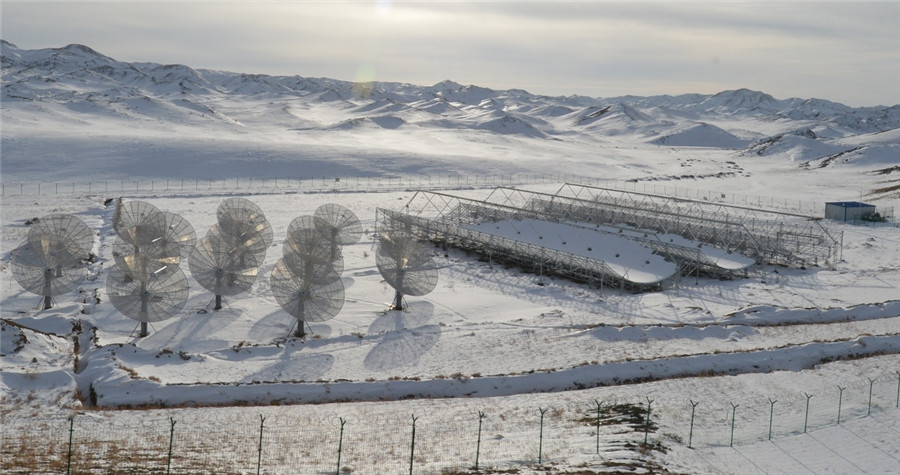
\includegraphics[width=0.9\textwidth]{./picture/Tianlai.jpg}
 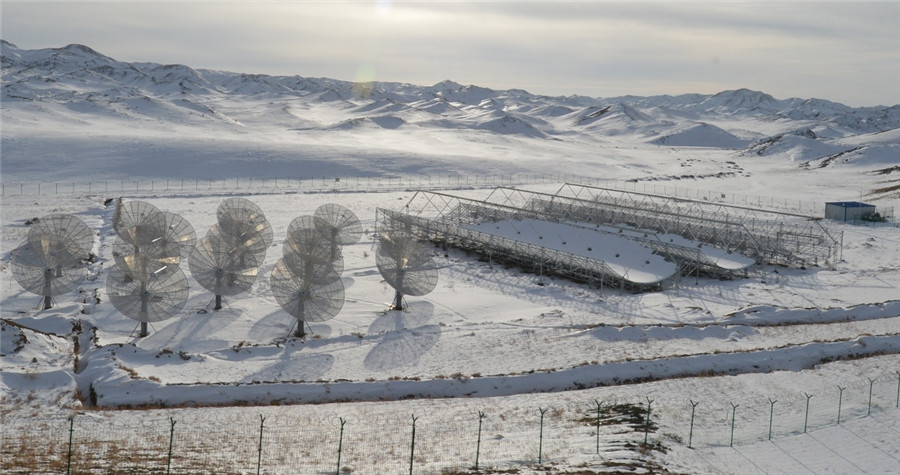
\includegraphics[width=0.9\textwidth]{./picture/Tianlai.jpg}
\caption{Tianlai interferometer Array. Left in the pitcture are 16 dishes telescope, right part are three cylinder telescopes.\label{fig:Tianlai}}
\end{figure}

\section{Whole System}\label{sec:1}
  

	ROACH2-GPU framework for correlator is popular in lots of radio interferometer array, like PAPER(Precision Array for Probing the Epoch of Re-ionization)\cite{2010AJ....139.1468P},LEDA(Large Aperture Experiment to Detect the Dark Ages) etc. Here we borrow the structure mainly from PAPER correlator model \cite{2008PASP..120.1207P}, and build up a flexible and scalable hybrid correlator system for Tianlai project.
	
	 For the whole correlator system, assuming F-engine has $M$ ROACH2 nodes,  X-engine has $N$ GPU nodes.  Every ROACH2 node handles  with $m$-way analog radio inputs, after FFT, outputs $m$ spectrums; each spectrum has $F$ frequency points. To optimize the data traffic, each GPU node only processes ${F}/{N}$ frequency points,  each frequency point includes $M\times m$ conjugate multiply computation. Therefore the ROACH node should divide the $F$ points spectrum into $N$ bands, then send specified band to corresponding GPU node. We will present the F-engine model in detail at \ref{sec:F-engine}. In GPU node ,  since GPU has $n$ cores,  the ${F}/{N}$ frequence points will be  distributed to $n$ cores to do conjugate multiply accumulation. We will introduce X-engine in detail at \ref{sec:X-engine}.            
	  
	The whole structure for Tianlai correlator is shown in Figure \ref{fig:structure}. The ROACH node could be controlled by ROACH2-server through Internet. Via a KATCP (Karoo Array Telescope Control Protocol) protocol, one could load the specified FPGA model to ROACH2 board.  We designed several FPGA models on CASPER(Collaboration for Astronomy Signal Processing and Electronics Research)  platform, for example, ADC raw data sample model which could output the digital data by sampling the analog signal directly, 32-input and 64-input model which are for the test of small scalar experiment based on PAPER model.  We also build up two different FFT length (1024 and 512) correlator models for different frequency resolution requirement of Tianlai. The six ROACH2 boads which are referred to as F-engine, sample 192-input analog signal from receiver with 8 bit resolution.  Then sampling digital data go through FFT, Equalizer, Transpose, 10Gb Ethernet functional blocks , finally reach 10Gb Ethernet switch. In switch part, each ROACH2 board has 4 10Gb Ethernet ports connected to switch, we assigned the static MAC address to each ports on switch and divide the network into several sub-network VLANs.  In X-engine, we implement distributed computational structure to do CMAC. We  have 8 GPU nodes to deal with different frequency bands. In each GPU node, we installed two GTX690 GPUs where there are two GPU cores in each GPU. Thus each GPU node can process conjugate multiply accumulation for 128  frequency points of 192 inputs.  We are using Hashpipe to manage thread and data transfer in each GPU node. 
		
	The required number of ROACH2 board is dependent on the number of antenna inputs. We have 2 ADC daughter boards installed in every ROACH2 board, while each ADC has 16 inputs.  If only consider the cylinder telescopes, we have 192 inputs, so 6 ROACH2 boards are needed.  The number of GPU nodes is determined by the computational intensity. As the result of testing for several times, The peak computational performance for each GPU core is 1.2 TFLOPS,  then each GPU node which have 4 cores has 4.8 TFLOPS peak computational performance. The total computational intensity for Tianlai pathfinder experiment is 35.6 TFLOPS. Therefore we presume  8 GPU nodes  could meet demand for present system.
\begin{figure}[t]
 \centering
 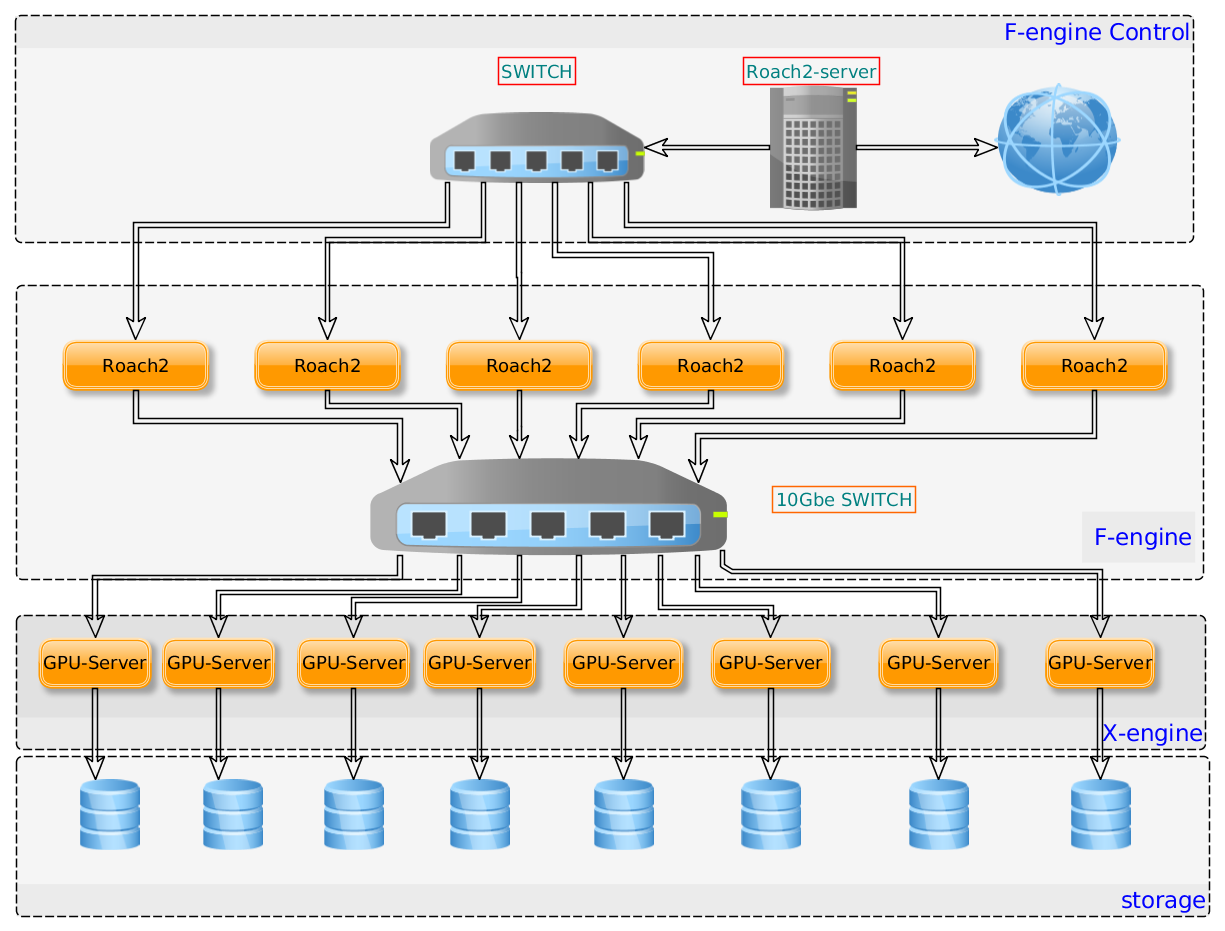
\includegraphics[width=0.9\textwidth]{./picture/structure1.eps}
\caption{Structure of Tianlai Correlator.\label{fig:structure}}
\end{figure}
\\
\subsection{F-engine}\label{sec:F-engine}
	F-engine model is built on CASPER platform. As a user of this platform, you don't need to pay more concentrations on FPGA code but only focus on the design of function for your model. Most ROACH2 hardware have their corresponding yellow Blocks which are already built by CASPER people\footnote{\url{https://casper.berkeley.edu/}}. It's quite convenient and efficient for astronomer or those who are in demand for FPGA implement but without a lot of FPGA language experience. In our correlator, F-engine is expected  to have ability of  converting analog to digital sample, FFT, frequency dependent data bits choosing,  and then sending different frequency band data of all antenna inputs to corresponding GPU node. We can realize these function  by dragging the blocks from CAPSER tools and deliberating the data interface, the delay and the data flow issue.

\subsubsection{Function Blocks\label{sec:function model}}
	The demand of Tianlai correlator is similar with PAPER correlator, We build our F-engine model based on PAPER F-engine model which are designed by David Macmahon. \citep{paper_correlator}. The whole function sketch is showed in Figure \ref{fig:f-engine}. As a radio-frequency interface,  2 16-input ADC daughter boards is mounted on ROACH2 board.  Each inputs will be sampled with 8-bit resolution then be transferred to PFB block. PFB block will mainly process FFT, before that there is a polyphase filter to input some window for less energy leakage in spectrum.
	
\begin{figure}[t]
 \centering
 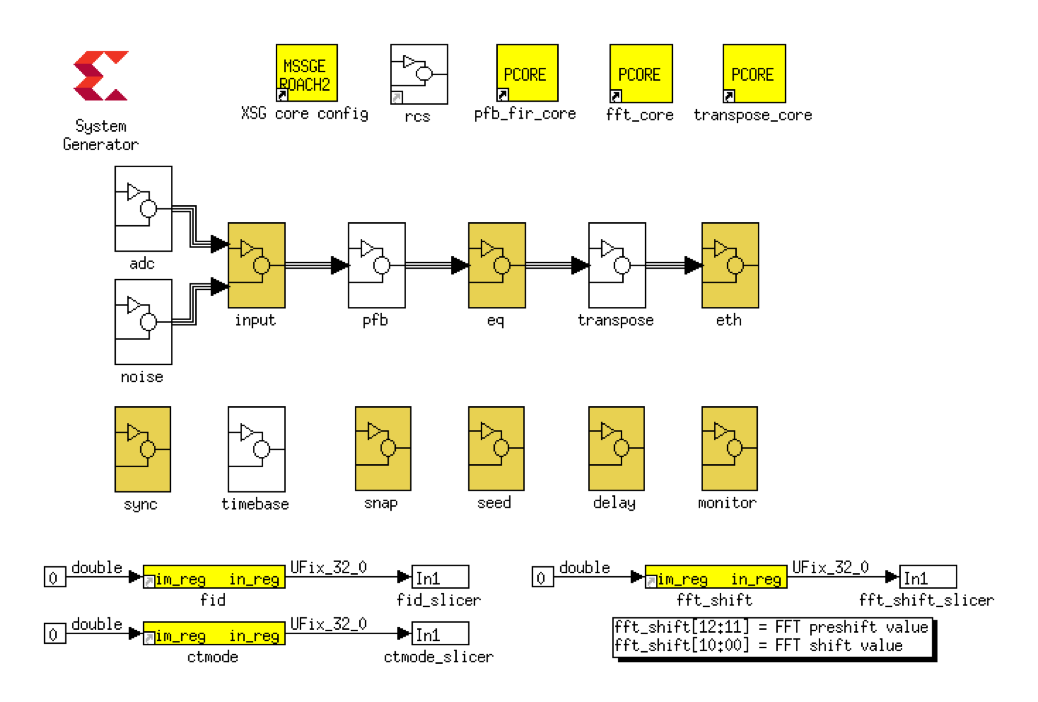
\includegraphics[width=0.9\textwidth]{./picture/f-engine1.eps}
\caption{F-engine model modified from PAPER correlator\label{fig:f-engine}}
\end{figure}


	To reduce the date exchange amount in the switch, we need to cut 18-bit data into 4 bits before sending to Ethernet.  However different receiver will have different frequency response, we use Equalizer block to take data bits at correct position and avoid wrong cut for different frequency channel. Each frequency channel of each input could have its own adjust factor. After Equalizer block, data flow for each input will become 4-bit real and 4-bit imaginary. 

\subsubsection{Transpose\label{sec:Transpose}}	
\begin{figure}[t]
 \centering
 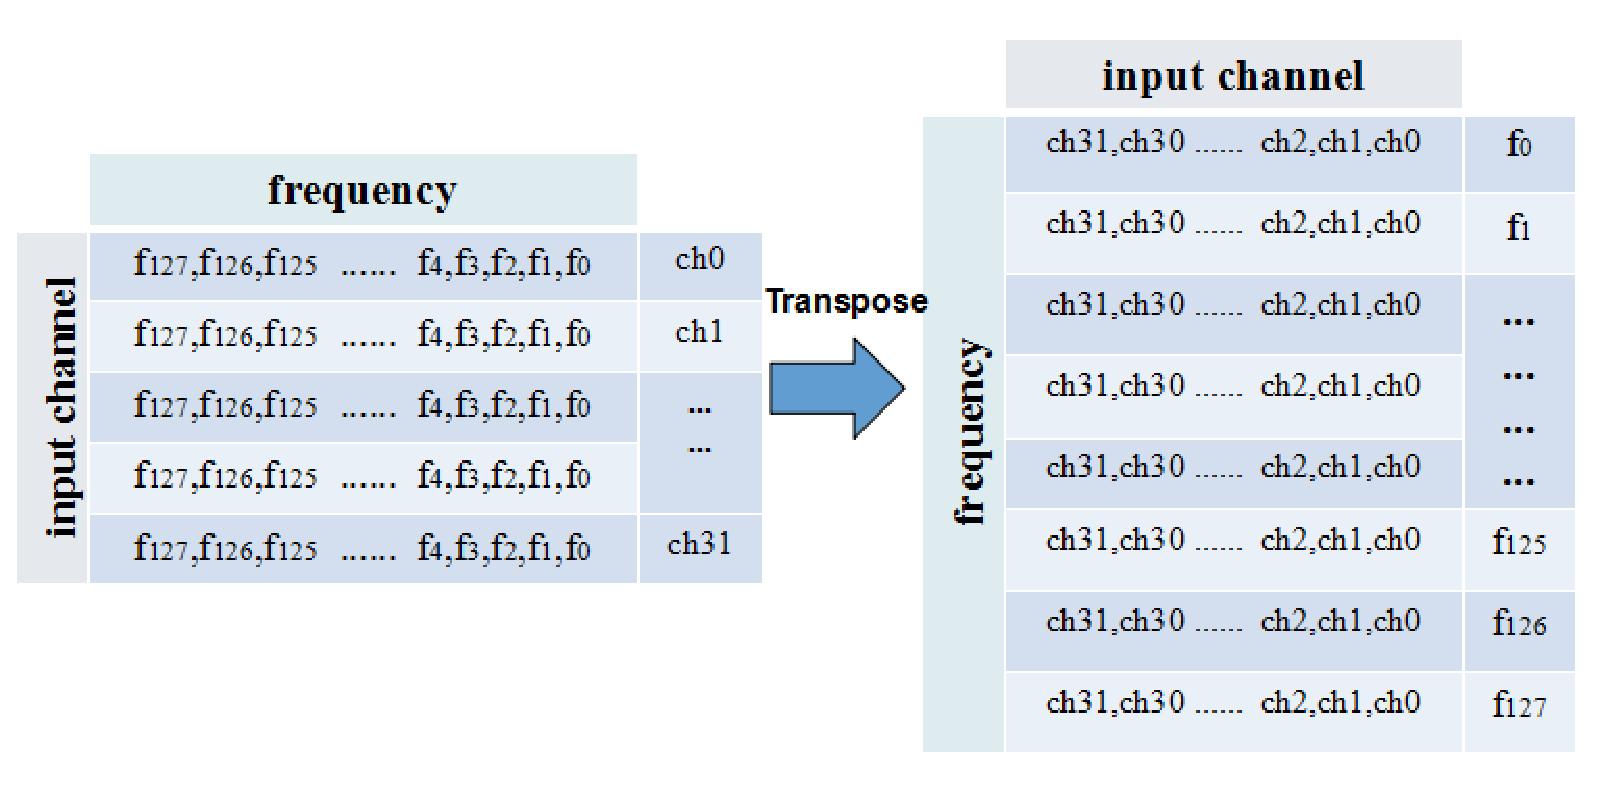
\includegraphics[width=0.9\textwidth]{./picture/transpose.eps}
\caption{Dataflow conversion of the Transpose. Left: Original data flow. Right: Transposed data flow.\label{fig:transepose}}
\end{figure}


   For the digital data after ADC and FFT, various frequency data of particular signal channel and time  is aranged in a succesive order in data flow,  however,  frequency channels must be distributed among a number of servers simultaniously, so suffering and making a transposition are mandatory before sending X engine with the frequency band data from all signal channels for a particalar time.  
	%As introduced in last section, different GPU node will process different part of frequency band from all antennas.  Before 
        %The different band are decided by F-engine Ethernet. but it also need to recognize that band is from which antenna input so that they could do conjugate multiply between inputs.
	%Voltage data go through FFT will become frequency points data flow, but each GPU node process one frequency band for all antenna inputs. 
        This need convert data shape from $[inputs,frequency]$ to $[frequency,inputs]$, like figure \ref{fig:transepose} shows. This operation could be achieved in a dual-port RAM through writing, reading from different address,\textcolor{red}{ alternative destination IP and changing header}.  Figure \ref{fig:transepose2} shows the overview of block design, if one output reading and writing address of dual-port RAM, we could see how exactly the reading and writing address change under flag signal from '$tid$','$fid$' etc.

\begin{figure}[t]
 \centering
 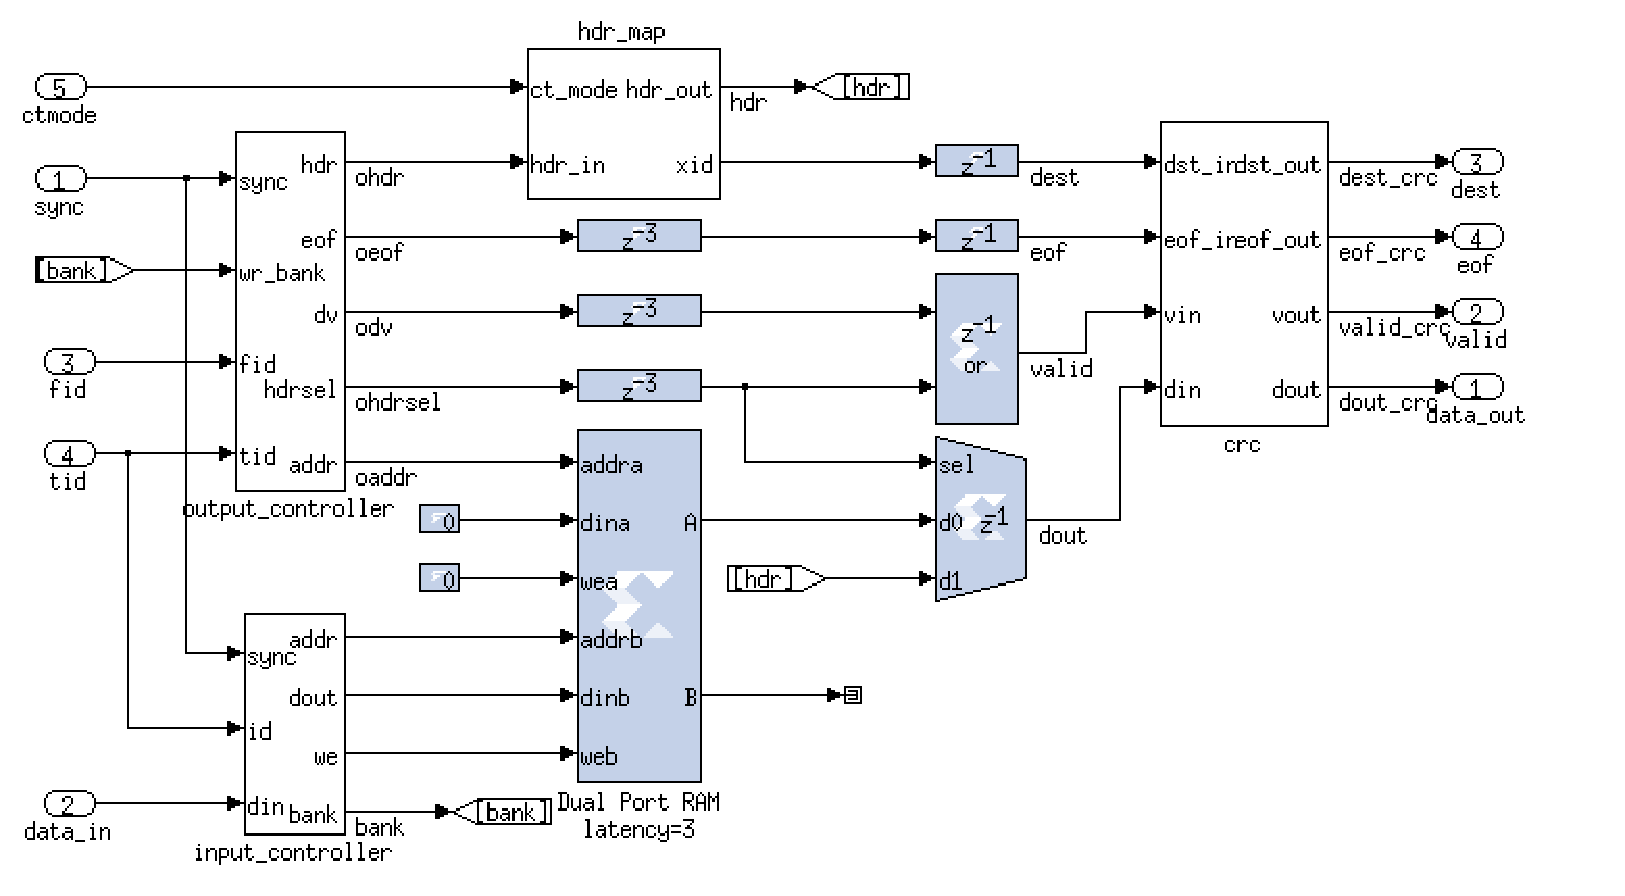
\includegraphics[width=0.9\textwidth]{./picture/transpose2.eps}
\caption{Structure of the second class sub-module in Transpose. One could modified dest IP and packet size in this model.\label{fig:transepose2}}
\end{figure}

%\begin{figure}
%\epsscale{1}
%\plotone{address1.png}
%\epsscale{1}
%\plotone{address2.png}
%\caption{The output of Writing and Reading address of Dual port RAM. Writing address varied with clock (uppder); Reading address varied with clock(bottom). \label{fig:address}}
%\end{figure}

Ethernet block is the last block on F-engine model. Models used on all ROACH2 nodes are the same. The only difference between ROACH nodes is IP and MAC configuration for Ethernet block. One ROACH2 node has four 10Gbps ports. Without using loopback mode in PAPER model, all the Ethernet ports are only sending but not receiving packets and each of them will have different IP \textcolor{red}{information} decided by '$tid$'. Detailed strategy for IP assignment will be described in sec \ref{sec:IP assignment}
	
When the F-engine Designed work is ready, one could simulate the design on Matlab with CASPER tools. After \textcolor{red}{De-bug} the model from simulation, we can generate a 'bof' file which could be uploaded to FPGA as firmware.
  
\subsubsection{Control System}

	Each ROACH2 node has been installed with a Power PC which can run simple linux system. The ROACH2 server has a service of  Network File System (NFS) which can share files, like the 'bof' files, with Power PC on ROACH2 node. Any time the ROACH2 boots up,  it will load the simple linux kernel from ROACH2 server or from onboard memory chip, which we called the booting methods as 'Net boot' or 'Solo boot' accordingly.  When whole system is running under Net boot, all ROACH2 boards will load the 'bof' files from NFS on ROACH2 server. 
	
        There are sync ports in all functional blocks in single ROACH2 node, The sync port will make sure every part inside model is \textcolor{red}{ready to run}. But between different ROACH2 nodes, the clocks are not synchronous. In this F-engine model design, there is a Sync model to sychronize all ROACH2 nodes on the same clock cycle. To achieve this, we connect 1PPS signal to each node. After all the parameters like IP, MAC address are set,  a sync signal which is called 'Arm signal' is sent to each node,  then all ROACH2 nodes will wait for the 1PPS signal to trigger the system. Arm signals at different nodes are not necessary to be sychronized at same time, but 1PPS signal are simultaneous by choosing the same length of cable.   After this operation, all the ROACH2 nodes will keep in the same pace. A diagram is showed in Figure \ref{fig:1pps}.
\begin{figure}[t]
 \centering
 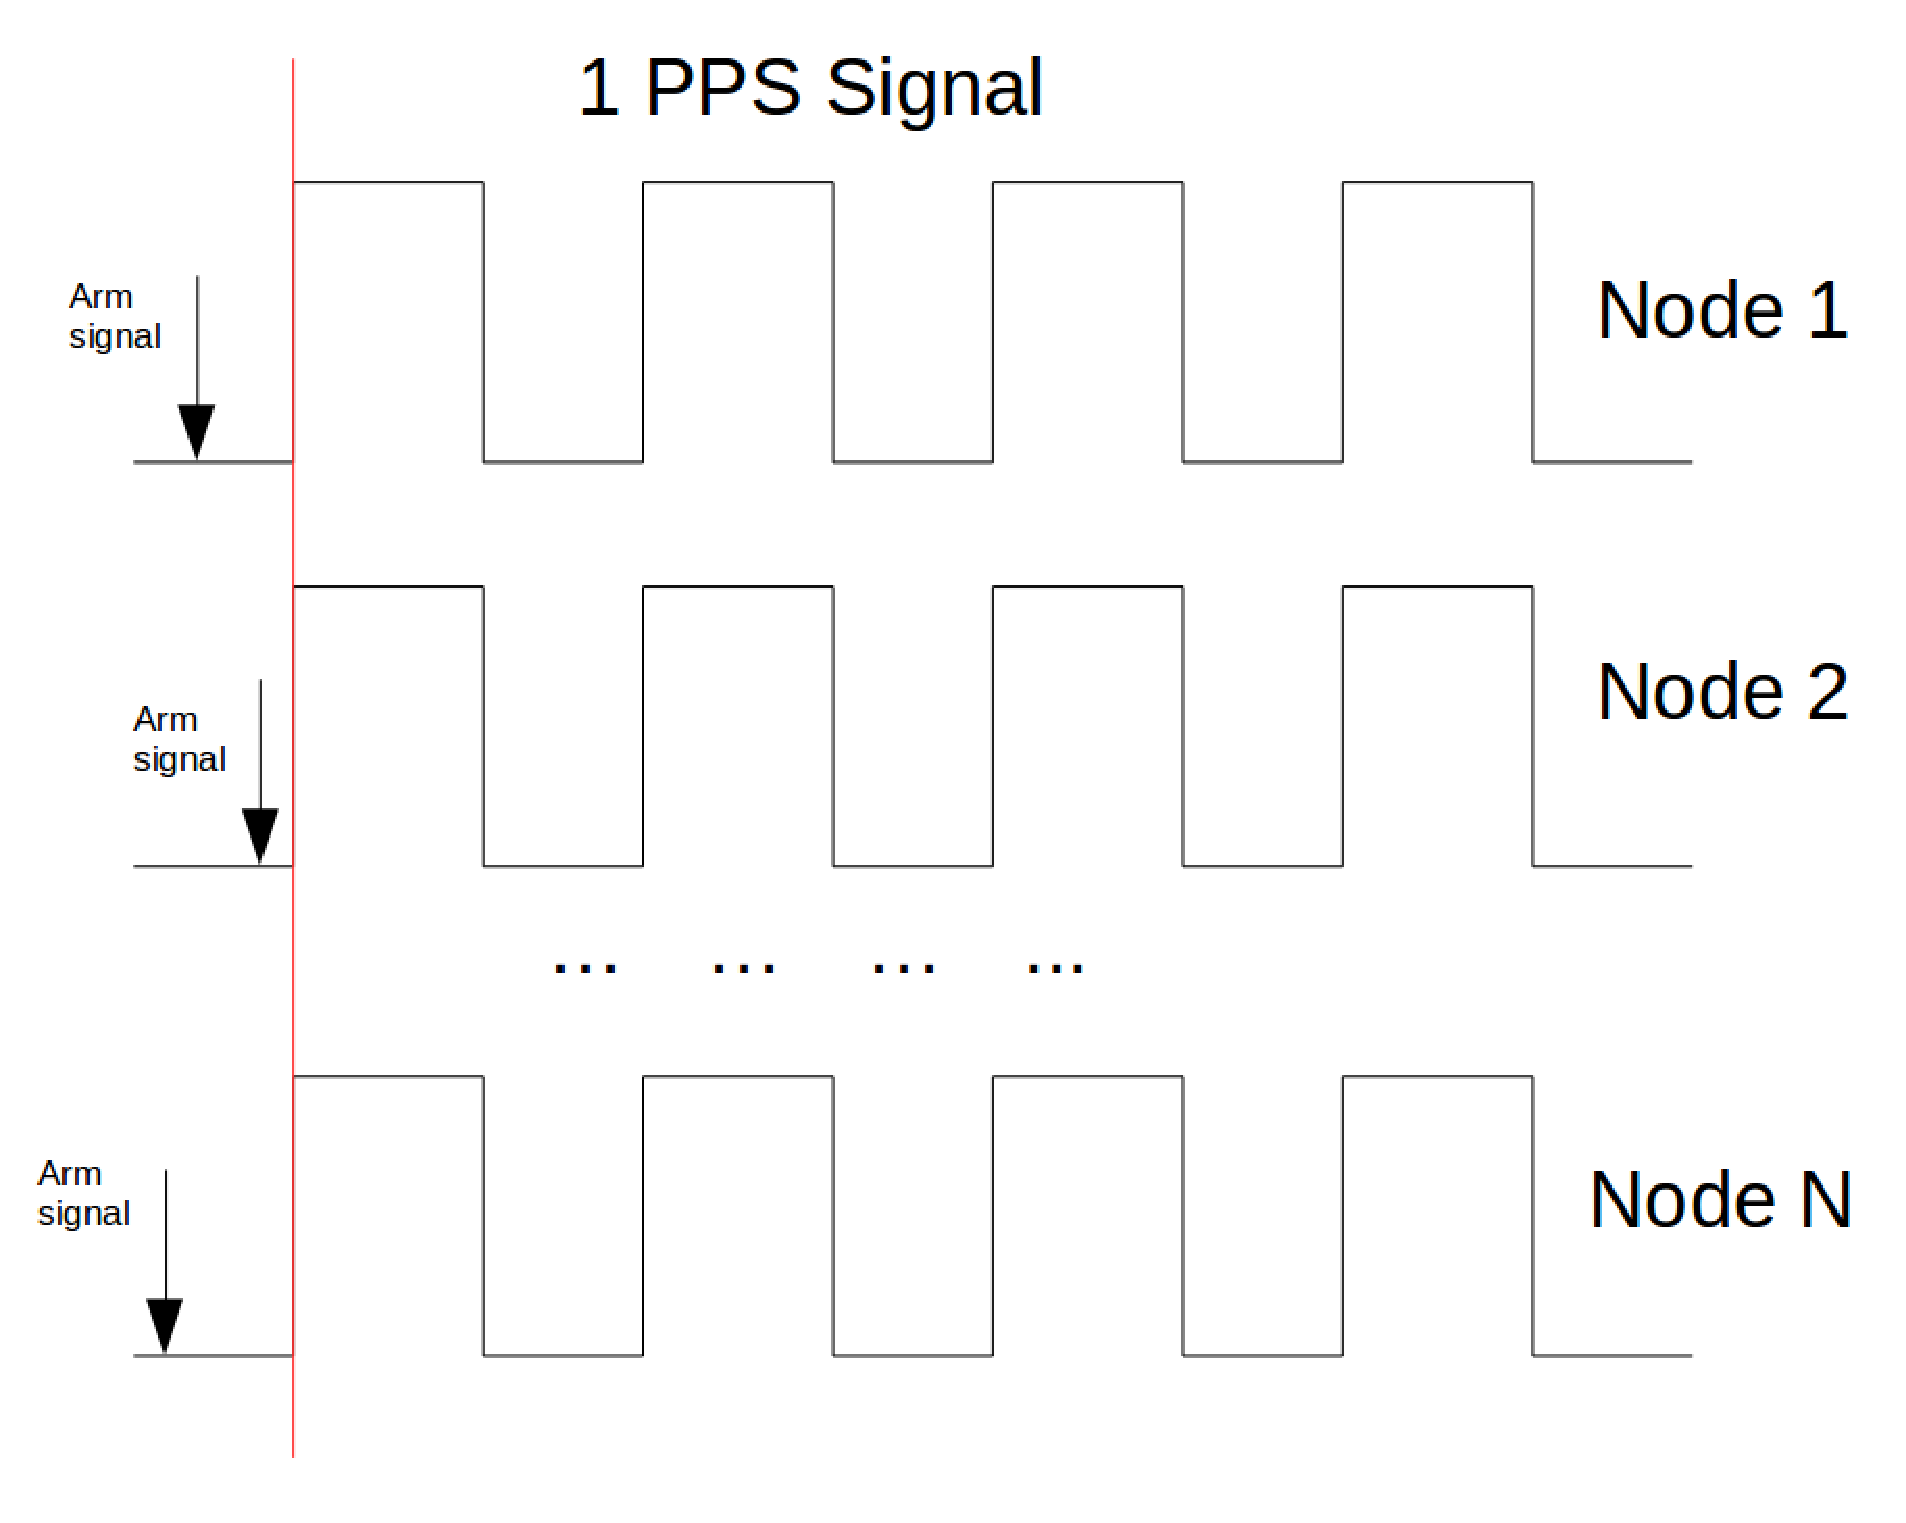
\includegraphics[width=0.5\textwidth]{./picture/1pps_sync.eps}
\caption{Synchronizing N ROACH2 nodes. The red lines indicate the start trigger using 1PPS signal\label{fig:1pps}}
\end{figure}


\subsection{X-engine}\label{sec:X-engine}

X-engine in this system is mainly responsible for  packets receiving, data distribution,  Conjugate Multiply Accumulation and  data storage. For one GPU node, there are 2 GTX690 cards where each have 2 GPU cores, 2 CPUs and four 10 Gbits NICs. These four GPU cores work separately, each of them will process CMAC of 32 frequency points. The CMAC process is using 'xGPU' package provided by Michael Clark etc. \cite{2013IJHPC..27..178C}.  'xGPU' code is written in CUDA-C and is optimized on GPU memory resources by specific thread tasks. It's designed originally to solve large array signal correlation process.

\subsubsection{Thread Manager:Hashpipe}	
	
	Data management in each GPU node are via Hashpipe\footnote{\url{https://github.com/david-macmahon/hashpipe}} which is developed by David MacMahon and Jeff Cobb etc.  Hashpipe specializes in communication among threads, moreover, it also could map CPU memory to GPU memory. In thread collaboration, data are stored in ring buffer between different threads. When ring buffer is filled by former thread, a warning message will be send to next thread. 

	The Hashpipe sketch is showed in Figure \ref{fig:hashpipe}, we open 4 threads and 3 ring buffers on each GPU node, each ring buffer is divided into 3 memory zone. Net thread is responsible for receiving data from  ROACH2 nodes, then resembles the data sequence required by xGPU code and stores data in GPU ring buffer. When ring buffer is full, the GPU thread starts to process the data in GPU ring buffer.  After GPU finished CMAC operation, it output the data in CPU ring buffer and clean GPU data buffer which are occupied by former Network thread data.  CPU thread adapted data structure to the form of final storage on disk, finally Disk thread write data to storage.
	Hashpipe also provide a status buffer which can extract key-value in each thread. This key-value will update in every running cycle. These status can be watched from a GUI monitor which have been written both in Ruby and Python. 
\begin{figure}[t]
 \centering
 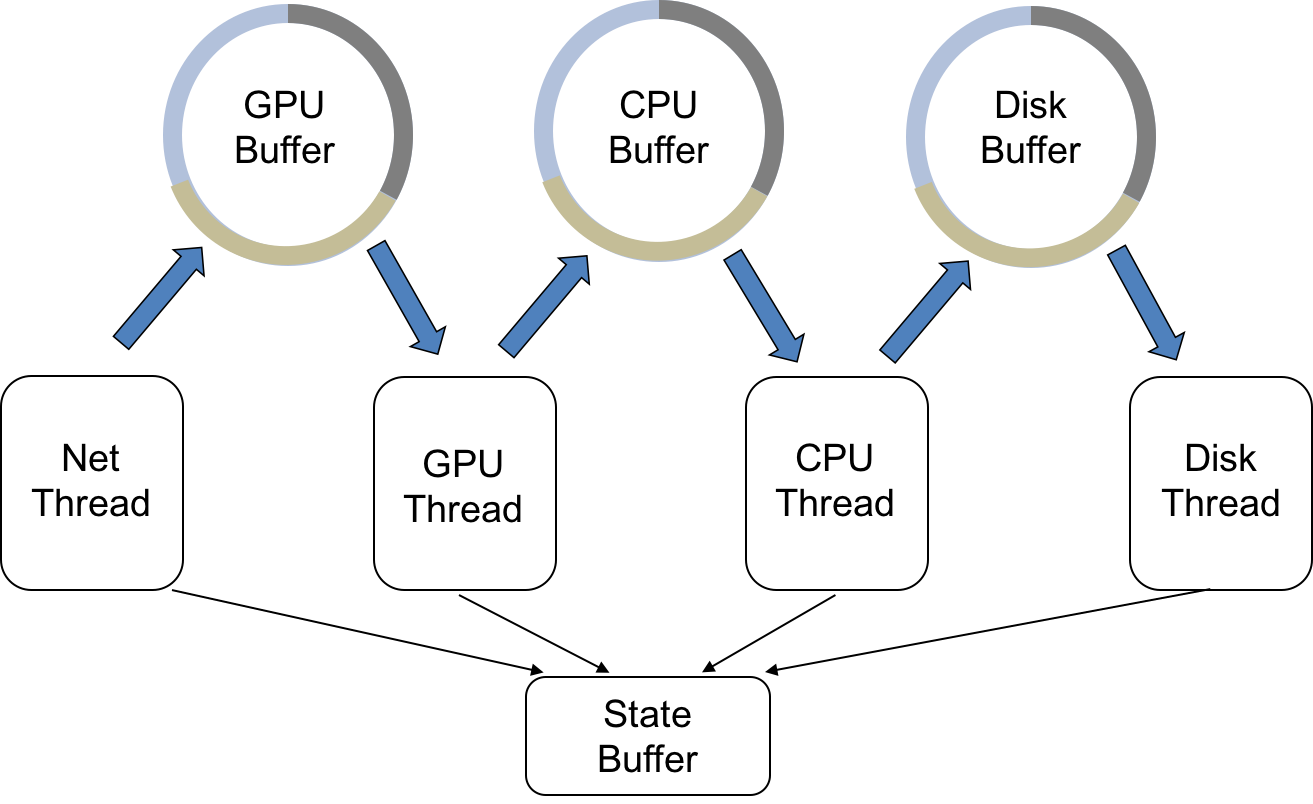
\includegraphics[width=0.7\textwidth]{./picture/hashpipe.eps}
\caption{Hashpipe thread manager structure.\label{fig:hashpipe}}
\end{figure}

\section{Local Network Framework \label{sec:Local Network}}
\subsection{Packet Formate \label{sec:Data formate}}
The Packet formate in this system is like Figure \ref{fig:data_formate}. The header part is 8 Bytes including 6 Bytes 'Mcnt' and 1 bytes for 'Fid' and 'Xid' separately. 'Mcnt' is used to count the packets number. At same time,'Mcnt' should keep same and coherent from different ROACH2 . The Hashpipe in X-engine will judge if loss packet from 'Mcnt' sequence. 'Fid' stand for F-engine ID and give an information of which ROACH2 node packet is from . Because every GPU node have four GPU cores, each will process $\frac{1}{N_{GPU}}$ of total band width,where $N_{GPU}$ stand for total GPU cores in the system. Here we have packets from 4 different source IP in one GPU node, each node use 'Xid' to know which GPU core the packet is going , meanwhile, which frequency band the packet is from. 
\begin{figure}[t]
\centering
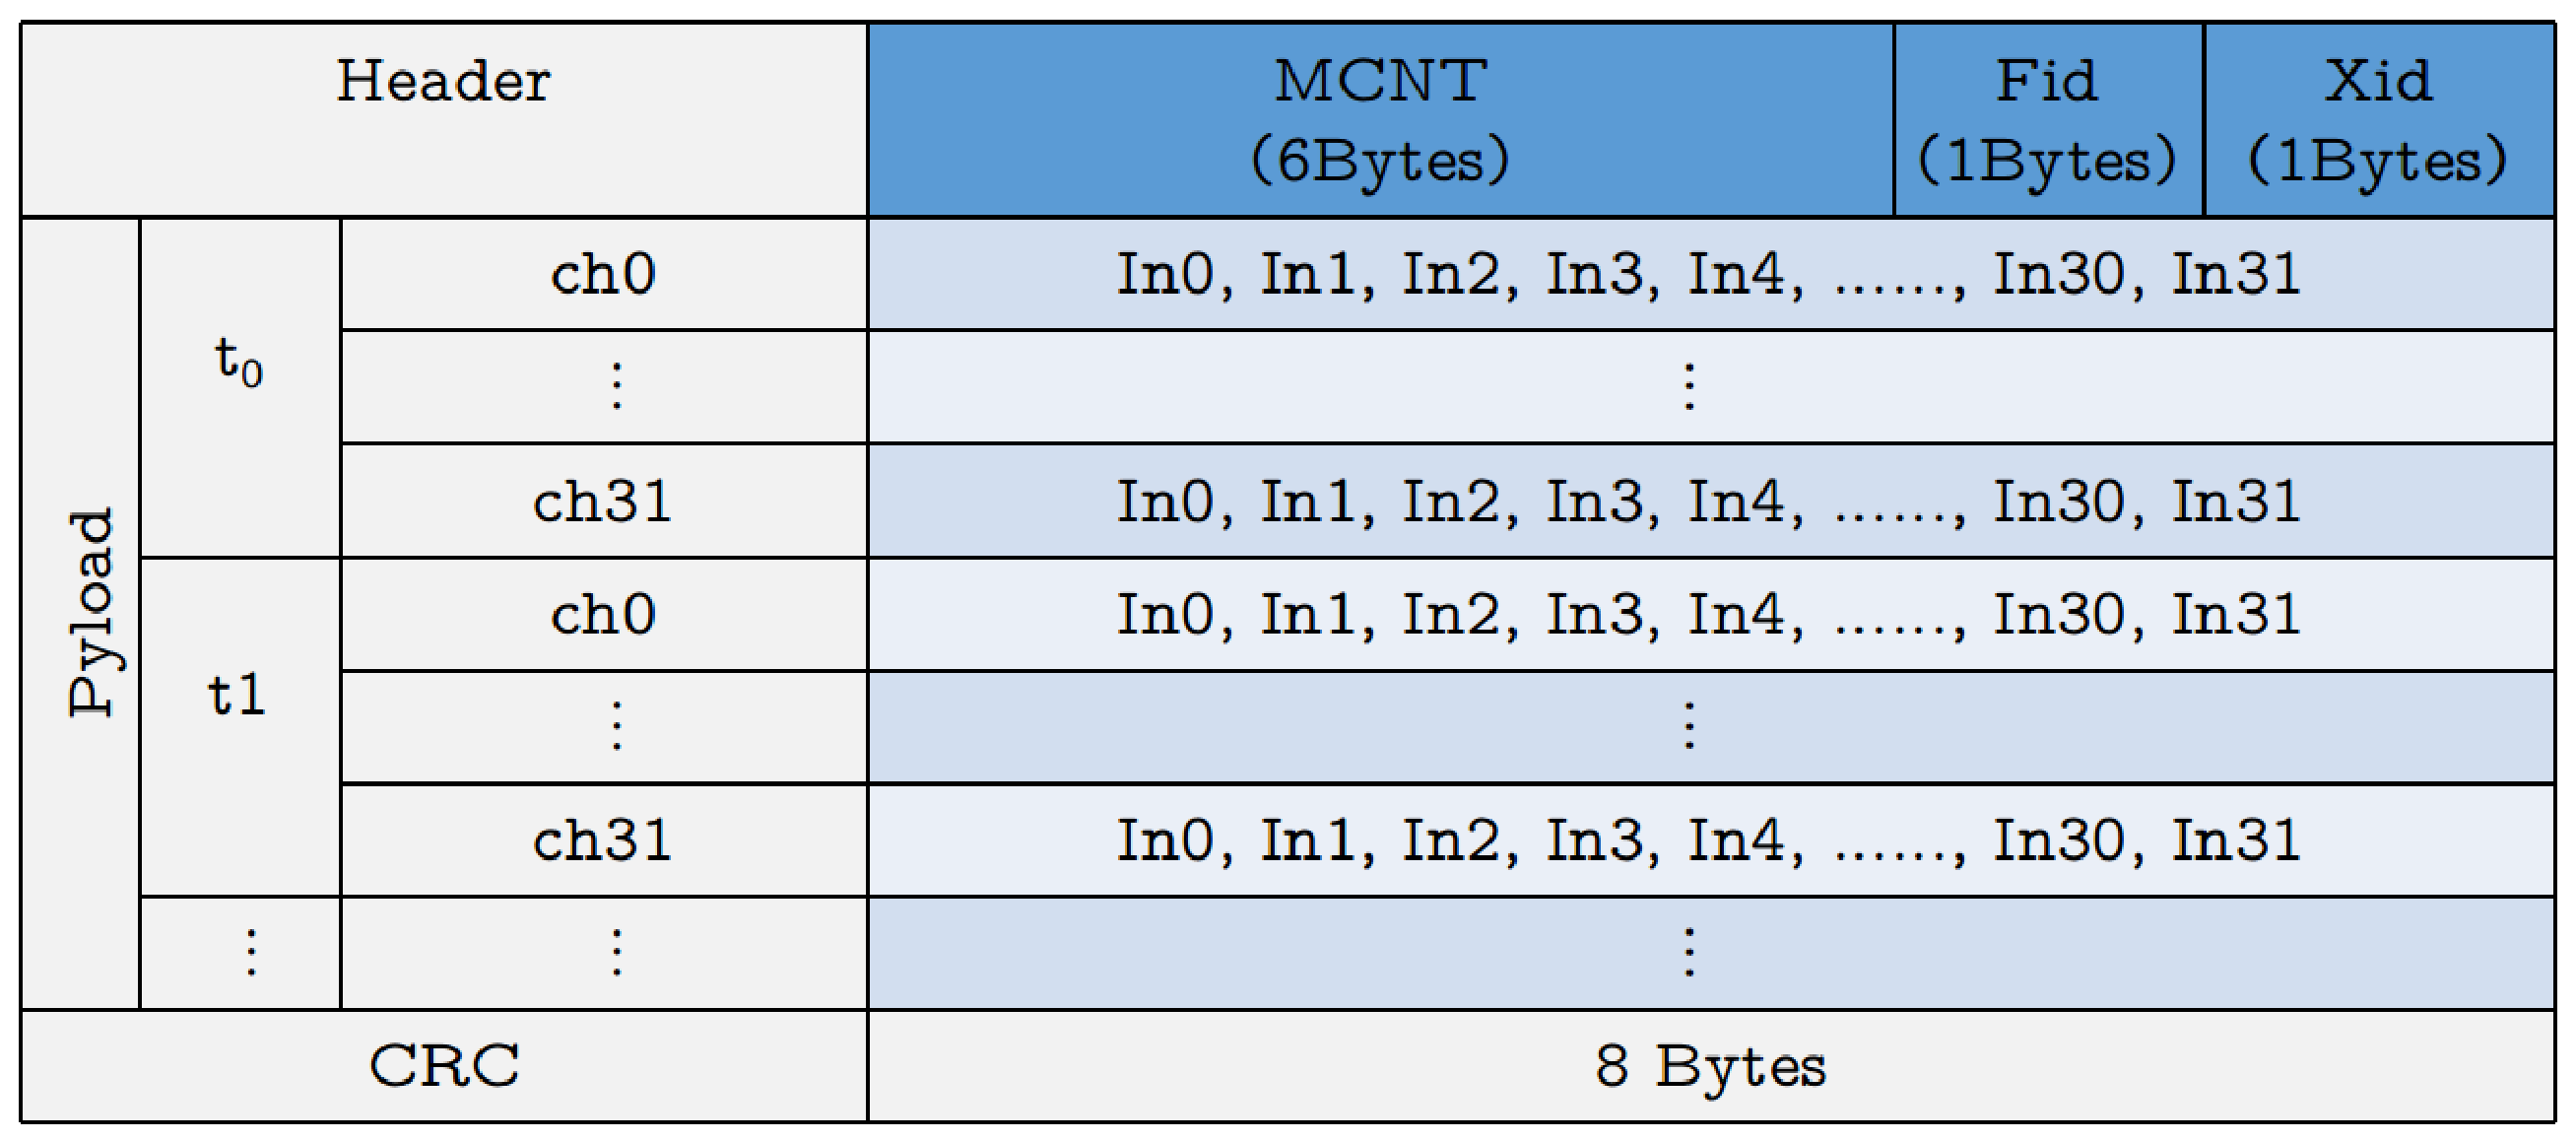
\includegraphics[width=0.9\textwidth]{./picture/Packet.eps}
\caption{Packet Data Formate in our system. For 512 FFT length model ,each time is from $ch0$ to $ch15$\label{fig:data_formate}}
\end{figure}

	Payload's data shape follows of $[time, channel, Input]$, In the Figure \ref{fig:data_formate}, 'In0' means data from input 0. The data from F-engine output is a complex number with 4 bits real part and 4 bits imaginary parts. There are $\frac{1}{32}$ frequency band equal $\frac{1024}{32}=32$ frequency channels in each packet. In order to optimize 10 Gbe data transfer, we add 8 times channels from next time stamp at same frequency band in each packet.  So the total size for one output packet from F-engine is:
\begin{equation} 
N_{chan}  \times N_{input} \times 8 + Header + CRC = 8208  (Bytes)
\end{equation}

\subsection{IP Assignment Strategy\label{sec:IP assignment}}
The junction between F-engine and X-engine is a 10 Gbe Switch. In our system, Every ROACH2 node have 4 10Gbe ports , and Each GPU node is also installed four 10 Gbe ports. So we total need $4\times 6 $ Roach2 nodes+ $4 \times 8 $ GPU nodes= 56 ports on  10Gbe switch. We apply Mellanox SX1024 Switch which have 48 ports of 10Gbe and 12 ports of 40Gbe. The 12 ports of 40 GbE can split into $12\times4=48$ ten GbE ports.

	Denote  $i \in[0,1,2,3]$ for 10 Gbe ports on each ROACH2 node. After transpose function model, the output from $i$ port of ROACH2 board will contains $\frac{BW}{4} \times i $ to $\frac{BW}{4} \times (i+1)$ frequency points which including 8 packets go to different GPU cores. Take port 0 for example, it has 0\--256 frequency points. As each GPU core process 32 frequency points, data out put from Port 0 should send to 8 GPU cores. Each GPU node has 4 GPU cores, so all the data from Port 0 will only go to GPU node0 and node1.  Thus we can put 10Gbe switch into 4 subnet using Vlan. Vlan1 are sub-net specific detour data from port 0 of each ROACH2 board to GPU node0 and node1. The packet got in GPU core will recognize the data source from the 'Fid' in Header, as introduced in section \ref{sec:Data formate}.
\begin{figure}[t]
 \centering
 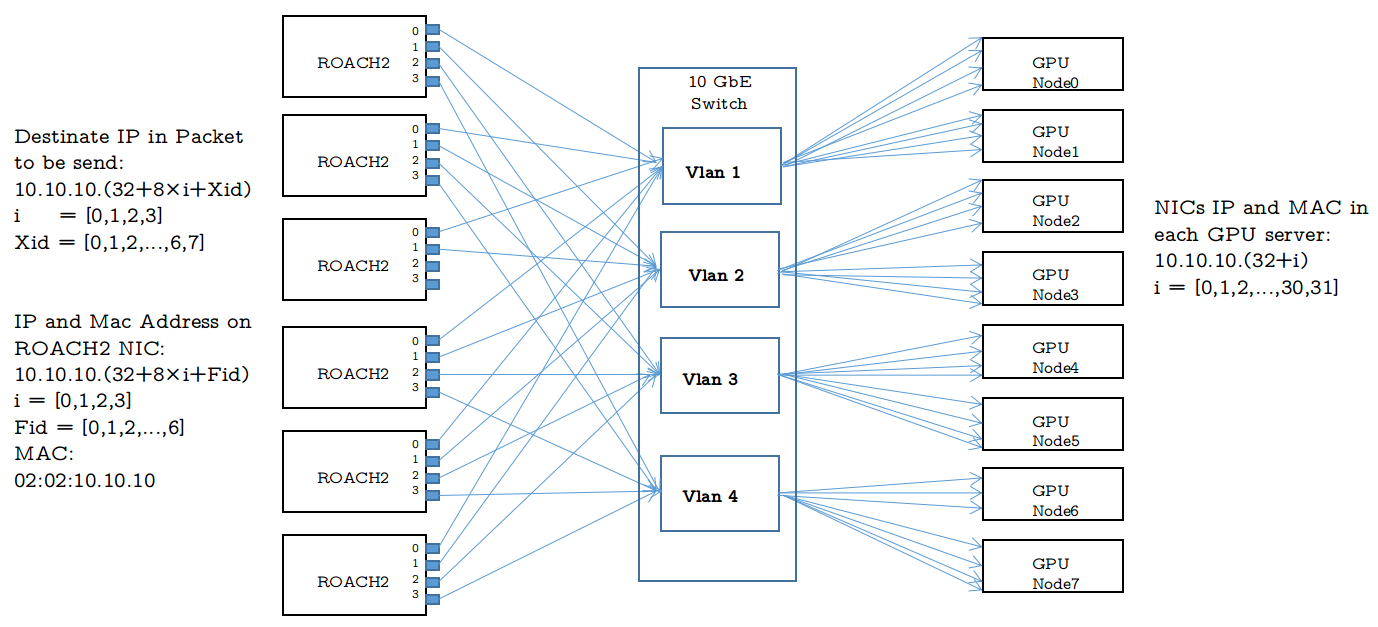
\includegraphics[width=0.9\textwidth]{./picture/Network.eps}
 \caption{Network and IP strategy in our system. We divide 10 Gbe Switch into four Vlans to avoid packets loss}
\end{figure}

\section{Experiment}\label{sec:experiment}
This system have been moved to our observatory site to take some experiments.  In the experiment, We have 6 roach2 but only 1 GPU node which have 4 GPU cores. Thus it just can handle 1/8 frequency band but from all inputs. 
\subsection{ADC and F-engine experiment}
We designed a ADC sampling model on ROACH2 which pack raw ADC samples directly and send to GPU server without doing FFT , Equalizer, Transpose etc. In this experiment, We input a 20MHz single tone analog signal to ADC . Then receiving Data from GPU node , we can output the digitalized signal and fitting it's frequency , the result we got is a sine wave with frequency 20.0001 MHz which bring an Error $10^{-6}$. 

%\begin{figure}
%\epsscale{1}[ht!]
%\plottwo{adc_sample.png}{sun.png}
%\caption{Left is ADC sample experiment. The blue dot is digitalized signal , Green line is fit data with unknow phase and frequency . The fresult frequency we got has a error %$10^{-6}$. Right one is phase between two telescope from observing of sun.%\label{fig:adc}}
%\end{figure}
We also did a frequency chirp test in F-engine, still input a single tone analog signal , after F-engine the signal will be in frequency domain. If we know the exact frequency of single tone wave input, we will get the relative position in frequency band. In GPU node, instead of Hashpipe , we use Wireshark to grasp the packet. In packet, we can see the data point shows in right place.
\subsection{Whole system test}
In correlation of two inputs, phase of visibility is depend on the signal time delay $\tau$ between two antenna. If input signal like $Ae^{i(2\pi ft + \phi)}$,  the two antenna with delay $\tau$ will have different inputs,  $Ae^{i(2\pi ft + \phi)}$ and  $Ae^{i(2\pi f(t+\tau) + \phi)}$, where $c$ is speed of light. After correlation , visibility is :
\begin{equation}
V = I_1^*\cdot I_2=Ae^{-i(2\pi ft + \phi)} \cdot Ae^{i(2\pi f(t+\tau) + \phi)} = I e^{i2\pi f\tau}
\end{equation}
Phase of visibility is $\Phi =(2\pi \tau )f$, it varied from $[-\pi, \pi]$.  When delay $\tau$ is a constant, phase will be linear with frequency, slope $k =2\pi \tau $. Here we did two experiments to generate time delay .  First one is to generate the simulate time delay by FPGA design, then add split Gaussian White Noise(GWN) into two inputs. This method will have exact time delay we already knew. Here we add $2.5\times 10^{-8}$s time delay, the slope in theoretical is $k=1.571\times 10^{-7}$rad/Hz. The $k_c$ got from correlator is $k_c = 1.561 \times 10^{-7}$ rad/Hz, error is $0.6\%$.
The other experiment we did is put a $7.5m$ radio cable to play as distance between two input signals.  As we know the speed that radio signal transit in radio wire is not exact speed of light. In this method ,we got the speed signal travel in wire is 0.7 speed of light. It is in reasonable range.
\subsection{Observation Test}
We have used this correlator observed Sun and Cygnus A and other radio sources. It's able to observe the interference fringe caused by the source move. We also take a collaborative observation with another correlator build by Institute of Automation,Chinese Academy of Sciences. Compare the phase varied by time, The result is almost the same. Figure \ref{fig:sun} shows the observation from sun, the phase fringe is obviously to see.
\begin{figure}[t]
 \centering
 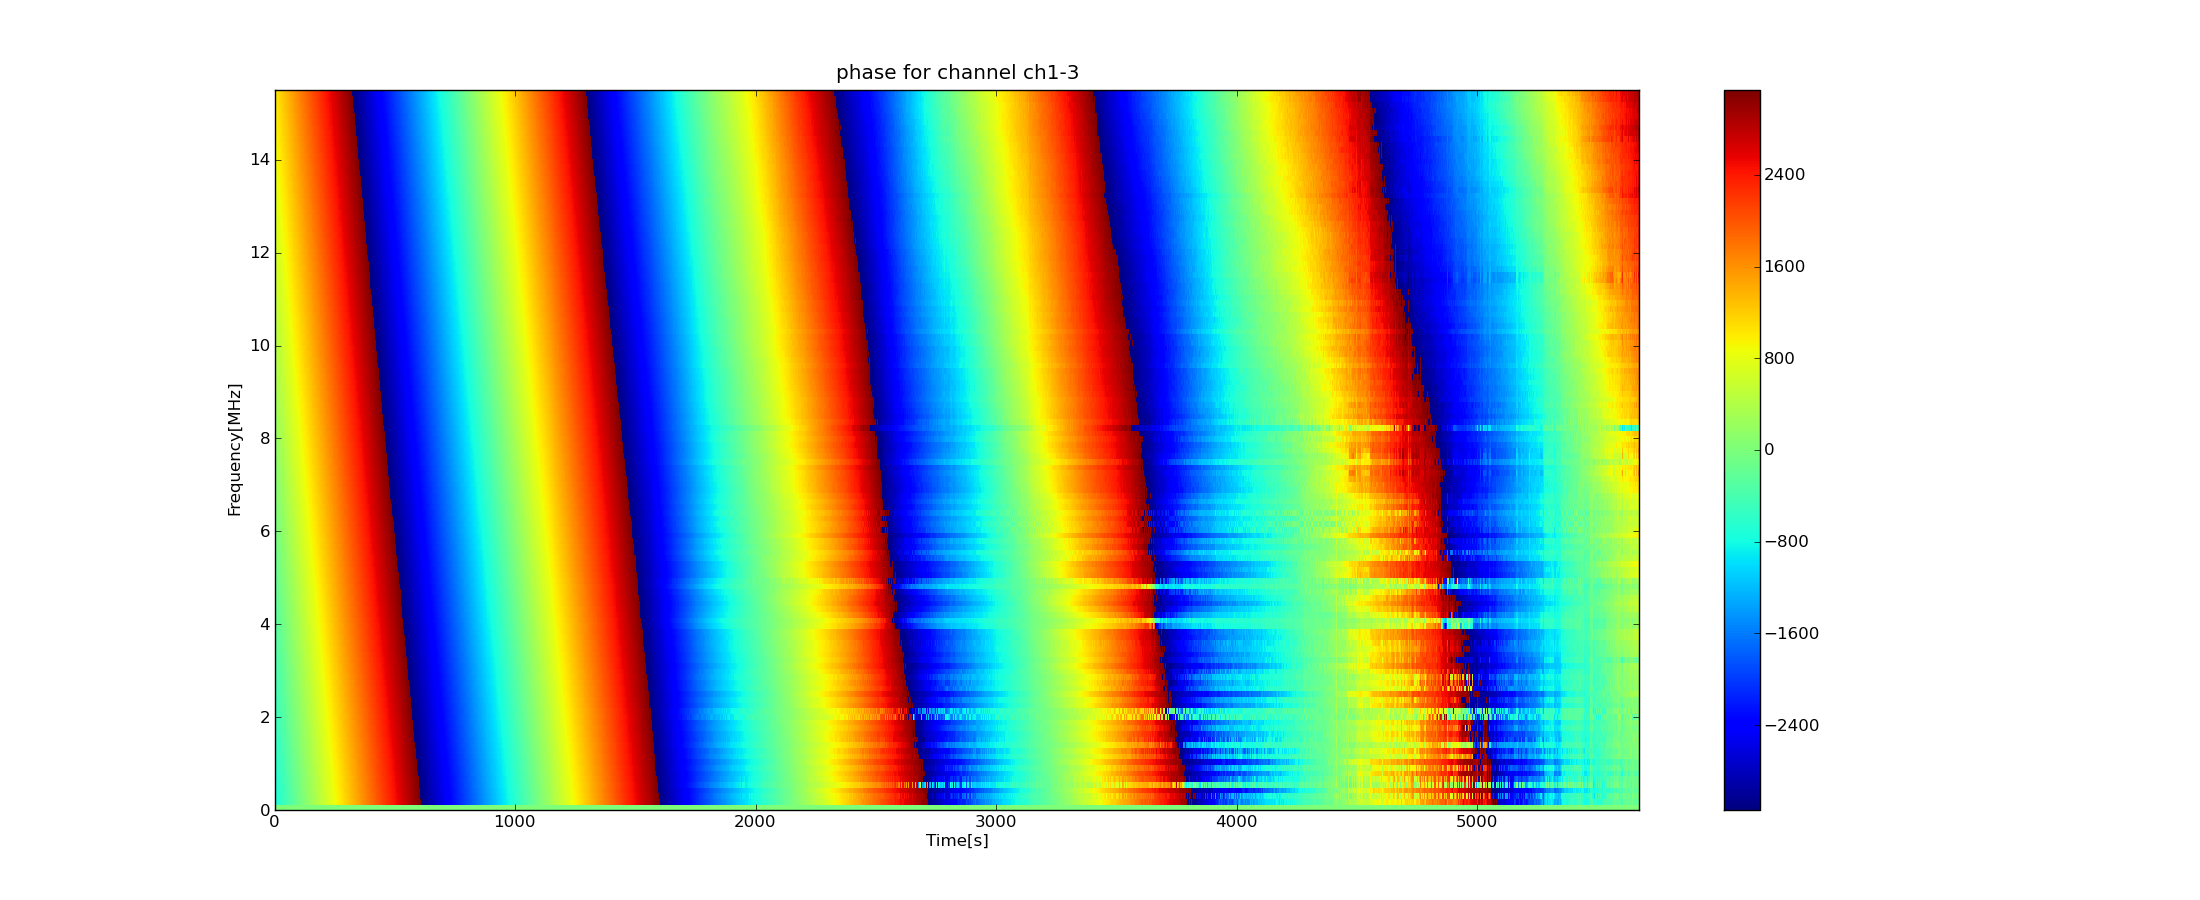
\includegraphics[width=0.9\textwidth]{./picture/sun.eps}
\caption{Phase fringe between two telescope inputs by observing of sun.\label{fig:sun}}
\end{figure}
\section{Sumarry}\label{sec:summary}	
This correlator system based on ROACH2-GPU framework is more flexible. We designed 1024 and 512 FFT length for different frequency resolution , and ADC sampling model to store the raw data sampled by ADC. In this correlator, F-engine gateware are same in different ROACH2 node. If  compute ability of X-engine is satisfied and have enough 10 Gbe ports on Switch. We could enlarge the antenna inputs simply by adding the ROACH2 nodes, the only difference is IP and Fid configuration for each ROACH2 board. The ROACH2-SWITCH-GPU framework could also used for different purposes at same time. Because Switch have a broadcast mechanism, When we need to extend the spectrum data from F-engine to other back-end like FRB back-end, this can be easily achieved by change the Switch configuration and connect the network cable to switch. We developed a special Models for Tianlai Array, But this system is easy to transplant to other telescopes with different demand like we did from PAPER model. We also did some premier experiment about our instrument, the correlator system is working normally. In the future, when our whole telescope complete, the same correlator can be use transplant easily. 


\bibliographystyle{ws-jai}
\bibliography{journals,Tianlai_correlator}


\end{document}
